
    \begin{frame}[fragile]{Industrial Logistics}
        The {\bf industrial logistics} is the process of {\bf planning}, {\bf organization}
        and {\bf control} of all the activities of handling and {\bf storage} of goods, which, starting
        from the suppliers and reaching up to the end user, guarantee an adequate
        level of {\bf service} to the customer consistent with the {\bf costs} to it associated

        \begin{figure}[hbt]
            \centering
            
\includegraphics[width=\textwidth]{img/ind4.png}
        \end{figure}
    \end{frame}

    \begin{frame}[fragile]{Multi-Robot Systems for logistic applications}

        \begin{figure}[hbt]
            \centering
            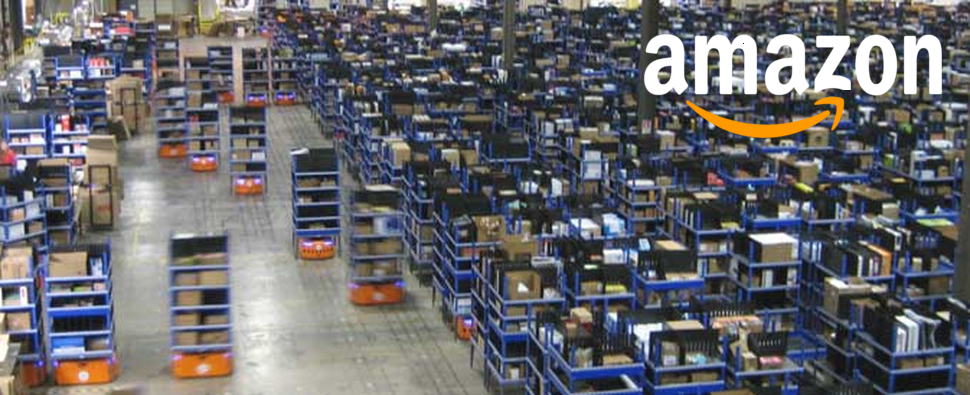
\includegraphics[width=\textwidth]{img/kiva.png}
        \end{figure}
        
        \begin{center}
        {\bf Kiva} warehouse-management system.
        \end{center}
    \end{frame}

    \begin{frame}[fragile]{Thesis contribution}
        \begin{center}
        The contribution of this thesis:
        \end{center}
        \begin{columns}
            \begin{column}{.7\textwidth}
           
            \begin{itemize}
            \item extension of  \texttt{ROS}  package
            \item proposing three tequnique:
            \begin{enumerate}
                \item Single robot : Single task (SR:ST) 
                \item Set Partition Strategy - Single robot : Multiple task (SPS1:N)
                \item Greedy Set Partition Strategy - Single robot : Multiple task (GSP1:N)
            \end{enumerate}
                \item real scenario: Computer Engineering for Industry 4.0 Laboratory (ICE Lab) 
            \end{itemize}
            \end{column}
            \begin{column}{.4\textwidth}
            \begin{figure}
                \subfloat{
\includegraphics[scale=0.45]{img/ros}}\qquad
                \subfloat{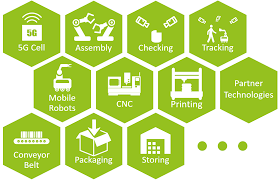
\includegraphics[scale=0.45]{img/ice}}
            \end{figure}
            \end{column}
        \end{columns}
    \end{frame}


    \begin{frame}[fragile]{ICE Laboratory}
        \begin{figure}[hbt]
            \centering
            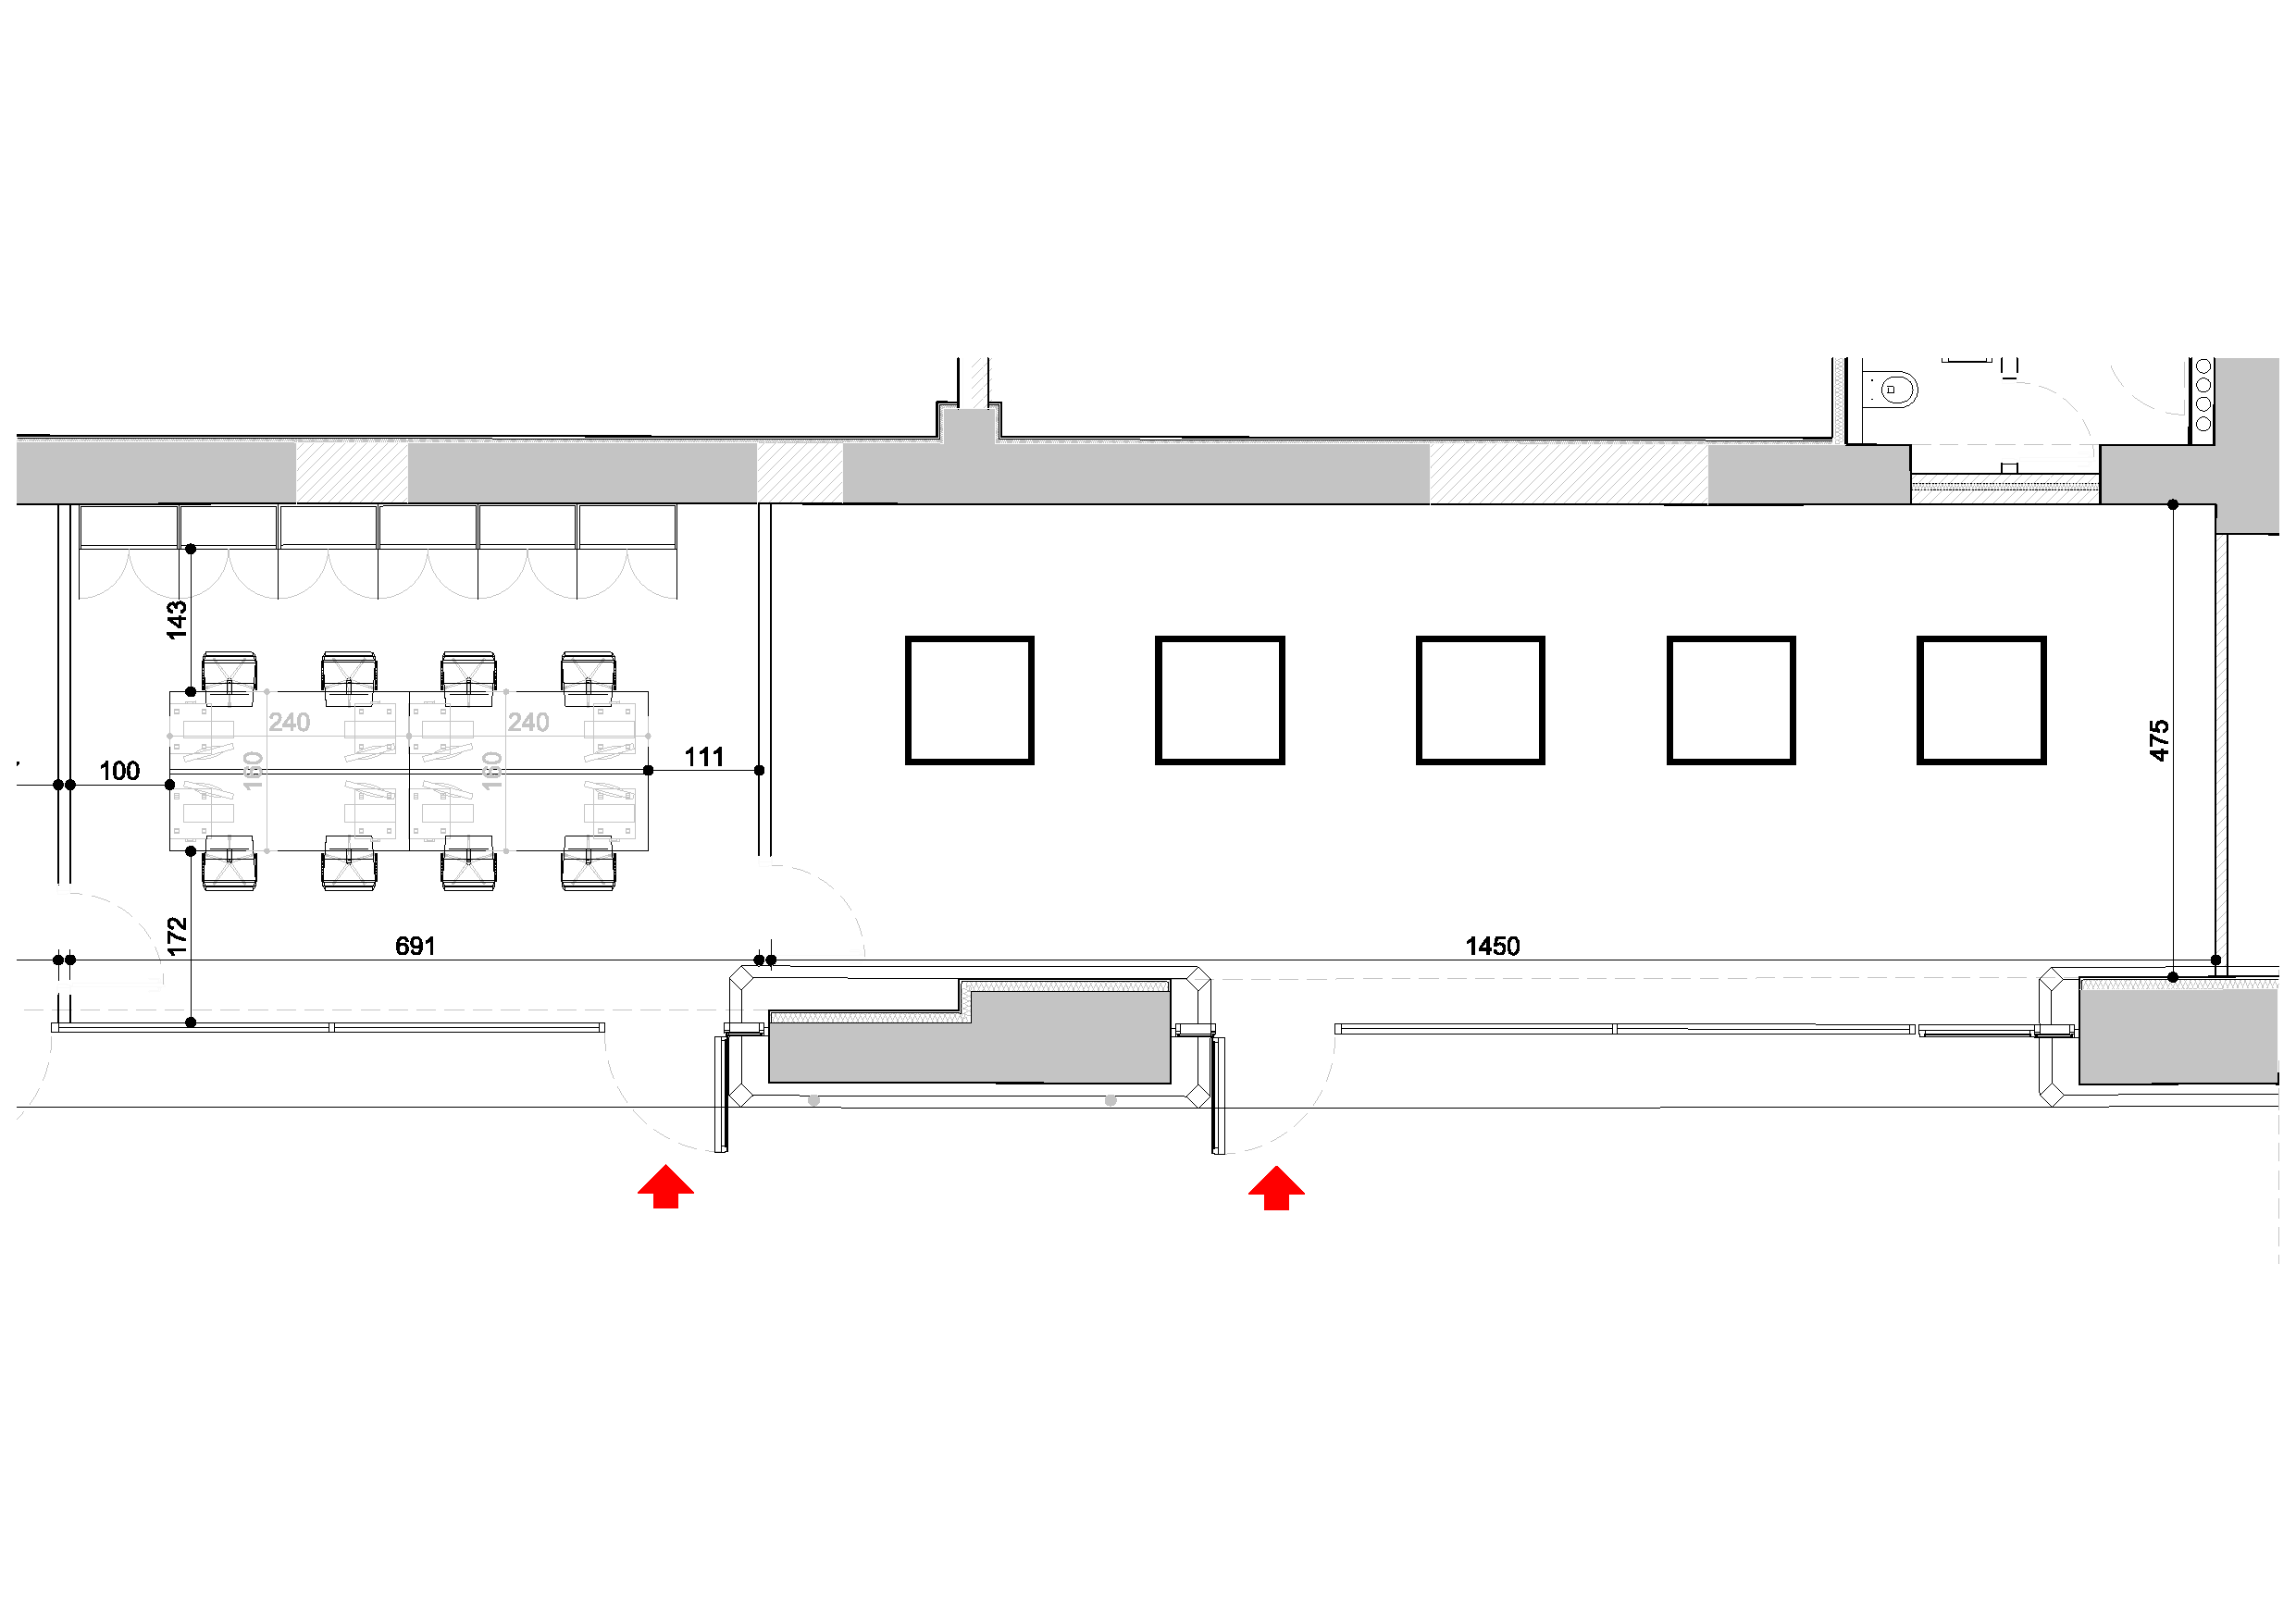
\includegraphics[width=\textwidth]{img/model1}
        \end{figure}
    \end{frame}

    \begin{frame}[fragile]{ICE Laboratory for logistic application}
        \begin{figure}[hbt]
            \centering
            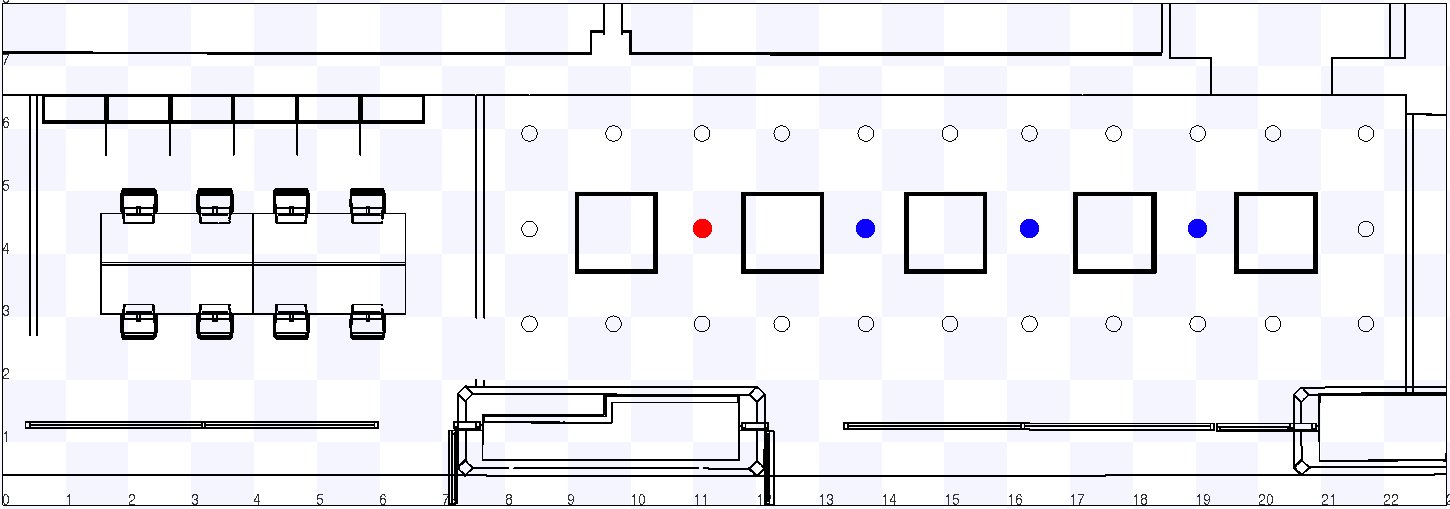
\includegraphics[width=\textwidth]{img/labgrafo}
        \end{figure}

        {\color{red}{$\bullet$}}  Loading bay
        \\
        {\color{blue}{$\bullet$}}  Unloading bays
        \\
        {\color{black}{$\circ$}}  Vertices
    \end{frame}

    \begin{frame}[fragile]{Problem formalization}
        Given a set of tasks $\mathcal{T}$ it defines intrinsically a set of orders $O$.
        One order perform a subset $S$ of $\mathcal{T}$, $S\subseteq\mathcal{T}$.

        $S = \{T_1,\cdots,T_k\}$ for each element we {\bf combine} their paths $P$ to form
        a single path $\pi = \{v_1,\cdots,v_i\}$.
        \begin{figure}
           
                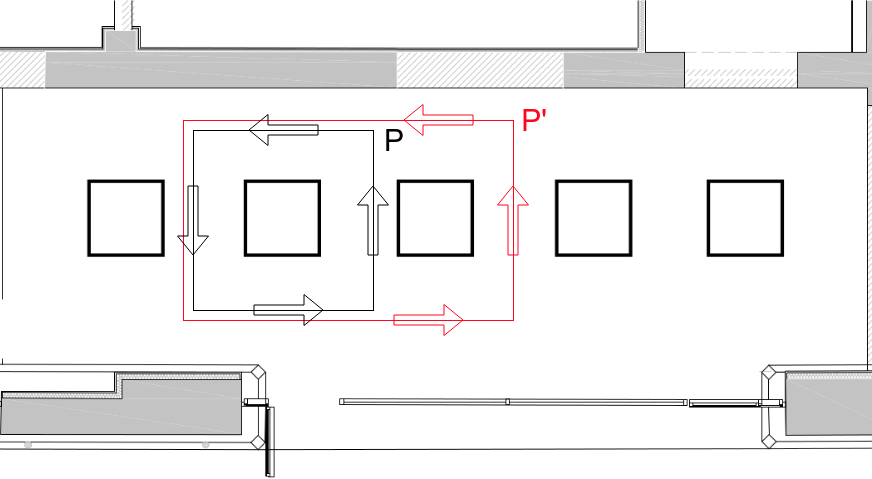
\includegraphics[scale=0.18]{img/p1p2_cut.png}
                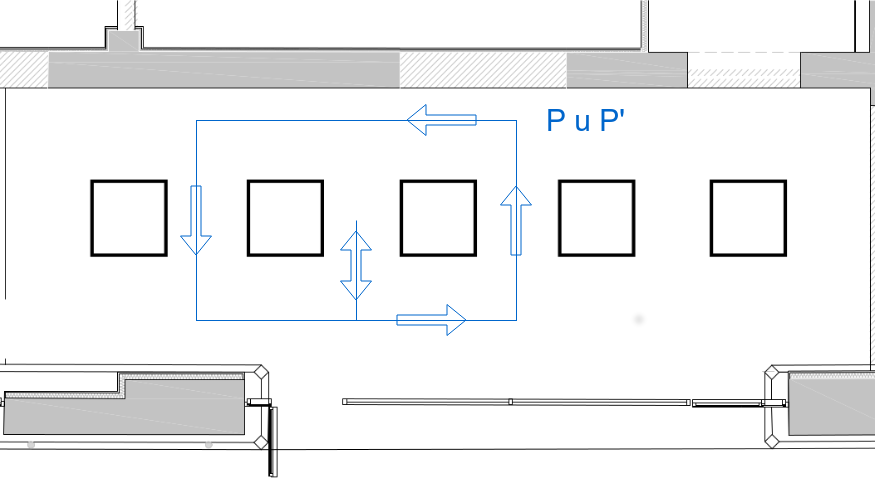
\includegraphics[scale=0.18]{img/p3_cut.png}

        \end{figure}
    \end{frame}

    \begin{frame}[fragile]{Problem formalization 2}
       We {\bf maximize} the total demand ($d_S$) we calculate the sum the single demand for each element in the subset.
\[d_S =demand(T_1) + \cdots + demand(T_k)\]
The heuristic function $v(\cdot)$ which
can be defined for any task $T$ or subset $S$:
\[ v(S) = \frac{f(\pi)}{d_S}\]

For compute the best partition of tasks the heuristic is based on the concept of {\bf loss} $L$,
which can be defined for any pair of subset $S_i$, $S_j$ as:
\[L(S_i,S_j) = v(\{ S_i \cup S_j\}) - v(S_i) - v(S_j)\]
where $v(S)$ is value of the characteristic function $v(\cdot)$ for subset $S$.

We want {\bf minimize} the cost of the {\bf loss}, that can be defined as:
\[L(S_i,S_j) < 0 \]
if the loss $L$ is less than 0 then we allocate the pair and delete the element which
form the subset.
    \end{frame}

    \begin{frame}[fragile]{Single robot : Single task (SR:ST)}
        This method is a {\bf baseline} for our logistic scenario.

        \begin{figure}[hbt]
            \centering
            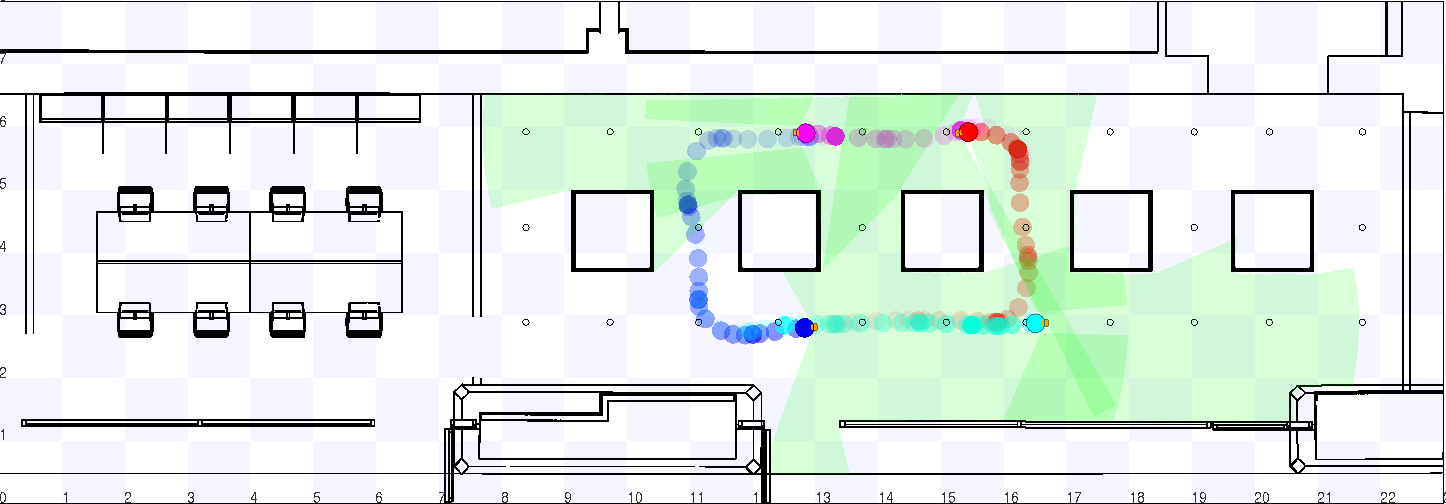
\includegraphics[width=\textwidth]{img/cycle1.png}
        \end{figure}
        The important constraint of this approach is to consider only {\bf one task} allocated for 
{\bf one robot} at time.
    \end{frame}

    \begin{frame}[fragile]{Set Partition Strategy - Single robot : Multiple task (SPS1:N)}
         \begin{columns}
            \begin{column}{.7\textwidth}
                \begin{center}
                    \begin{tabular}{|c|r|c|} \hline
                    \textbf{iteration} & \textbf{partition size} & \textbf{partition} \\ \hline
                    1    & 1    & \{\{a, b, c, d\}\}   \\
                    2    & 2    & \{\{a, b, c\}, \{d\}\}   \\
                    3    & 2    & \{\{a, b, d\}, \{c\}\}   \\
                    4    & 2    & \{\{a, b\}, \{c, d\}\}   \\
                    5    & 3    & \{\{a, b\}, \{c\}, \{d\}\}   \\
                    6    & 2    & \{\{a, c, d\}, \{b\}\}   \\
                    7    & 2    & \{\{a, c\}, \{b, d\}\}   \\
                    8    & 3    & \{\{a, c\}, \{b\},\{d\}\}   \\
                    9    & 2    & \{\{a, d\}, \{b, c\}\}   \\
                    10   & 2    & \{\{a\}, \{b, c, d\}\}   \\
                    11   & 3    & \{\{a\}, \{b, c\}, \{d\}\}   \\
                    12   & 3    & \{\{a, d\}, \{b\}, \{c\}\}   \\
                    13   & 3    & \{\{a\}, \{b, d\}, \{c\}\}   \\
                    14   & 3    & \{\{a\}, \{b\}, \{c, d\}\}   \\
                    15   & 4    & \{\{a\}, \{b\}, \{c\},\{d\}\}   \\ \hline       
                    \end{tabular}
                  \end{center}
            \end{column}
            \begin{column}{.4\textwidth}
            \begin{figure}
                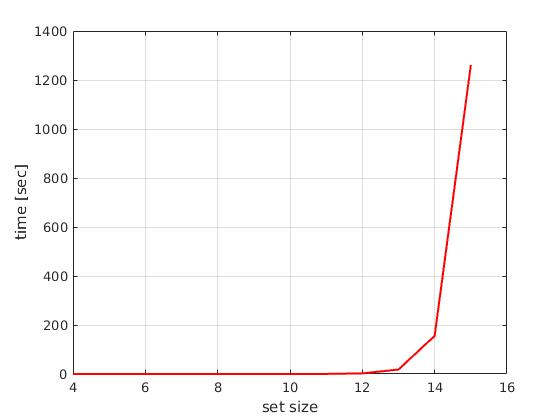
\includegraphics[width=\textwidth]{img/exp}
            \end{figure}
            \end{column}
        \end{columns}
    \end{frame}

    \begin{frame}[fragile]{Greedy Set Partition Strategy - Single robot : Multiple task (GSP1:N)}
        The main concept of this approach is composing tasks using Greedy {\bf Coalition Formation} strategy.
        \begin{figure}[hbt]
            \centering
            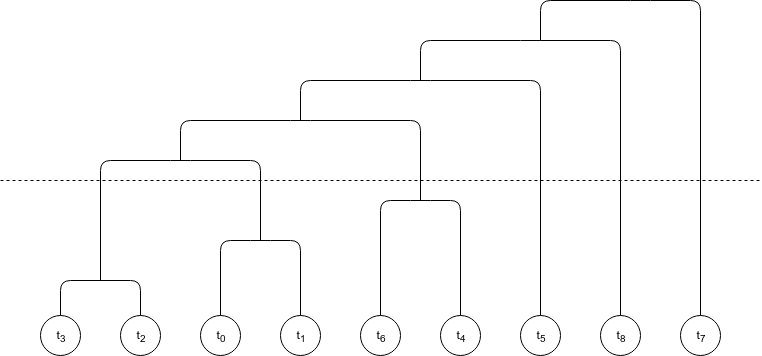
\includegraphics[width=\textwidth]{img/CF.png}
        \end{figure}
        The horizontal line represents a cut during execution it defines the coalition structure.
    \end{frame}

    \begin{frame}[fragile]{Example}
        Given a set of tasks $\mathcal{T}= \{  \{T_0\}, \{T_1\}, \cdots, \{T_8\} \}$ defined like:

        ${T_i=(item, demand, unloading\_bay)}$.
        
        The agents have the same capacity $C_{0,1,2,3} = 4$.
                    \begin{center}
                      % \centering
                      \begin{tabular}{|c|c|c|c|} \hline
                        \textbf{task} & \textbf{item} & \textbf{demand} & \textbf{unloading bay} \\ \hline
                        0    & A    & 1      & 0             \\
                        1    & B    & 2      & 1             \\
                        2    & C    & 3      & 2             \\
                        3    & A    & 1      & 0             \\
                        4    & B    & 2      & 1             \\
                        5    & C    & 3      & 2             \\
                        6    & A    & 1      & 0             \\
                        7    & B    & 2      & 1             \\
                        8    & C    & 3      & 2             \\ \hline       
                      \end{tabular} 
                    \end{center}
                    Often in the logistic environments robots are all equal. 
            
    \end{frame}

    \begin{frame}[fragile]{Example 2}
        Result SPS:
            \begin{center}
              \begin{tabular}{|c|c|c|c|} \hline
              \textbf{task} & \textbf{item} & \textbf{demand} & \textbf{unloading bay} \\ \hline
              \{4,7\}    & B    & 4     & 1             \\
              \{0,1,3\}  & \{A,B\}& 4    & \{0,1\}             \\
              \{2,6\}    & \{C,A\}    & 4  & \{0,2\}             \\
              5    & C    & 3      & 2             \\
              8    & C    & 3      & 2             \\ \hline       
              \end{tabular}
              
            \end{center}
   Result GSP:
            \begin{center}
              \begin{tabular}{|c|c|c|c|} \hline
              \textbf{task} & \textbf{item} & \textbf{demand} & \textbf{unloading bay} \\ \hline
              \{3,2\}    & \{A,C\}    & 4     & \{0,2\}             \\
              \{0,1\}    & \{A,B\}    & 3     & \{0,1\}             \\
              \{6,4\}    & \{A,B\}    & 3     & \{0,1\}             \\
              5    & C    & 3      & 2             \\
              8    & C    & 3      & 2             \\        
              7    & B    & 2      & 1             \\\hline
              \end{tabular}
              
            \end{center}
       
    \end{frame}

    \begin{frame}[fragile]{Video}
        \movie[height=6.5cm,width=11.5cm,loop]{}{video/video.mp4}
    \end{frame}

    \begin{frame}[fragile]{ROS package Logistic\_sim}
        \begin{figure}[hbt]
            \centering
            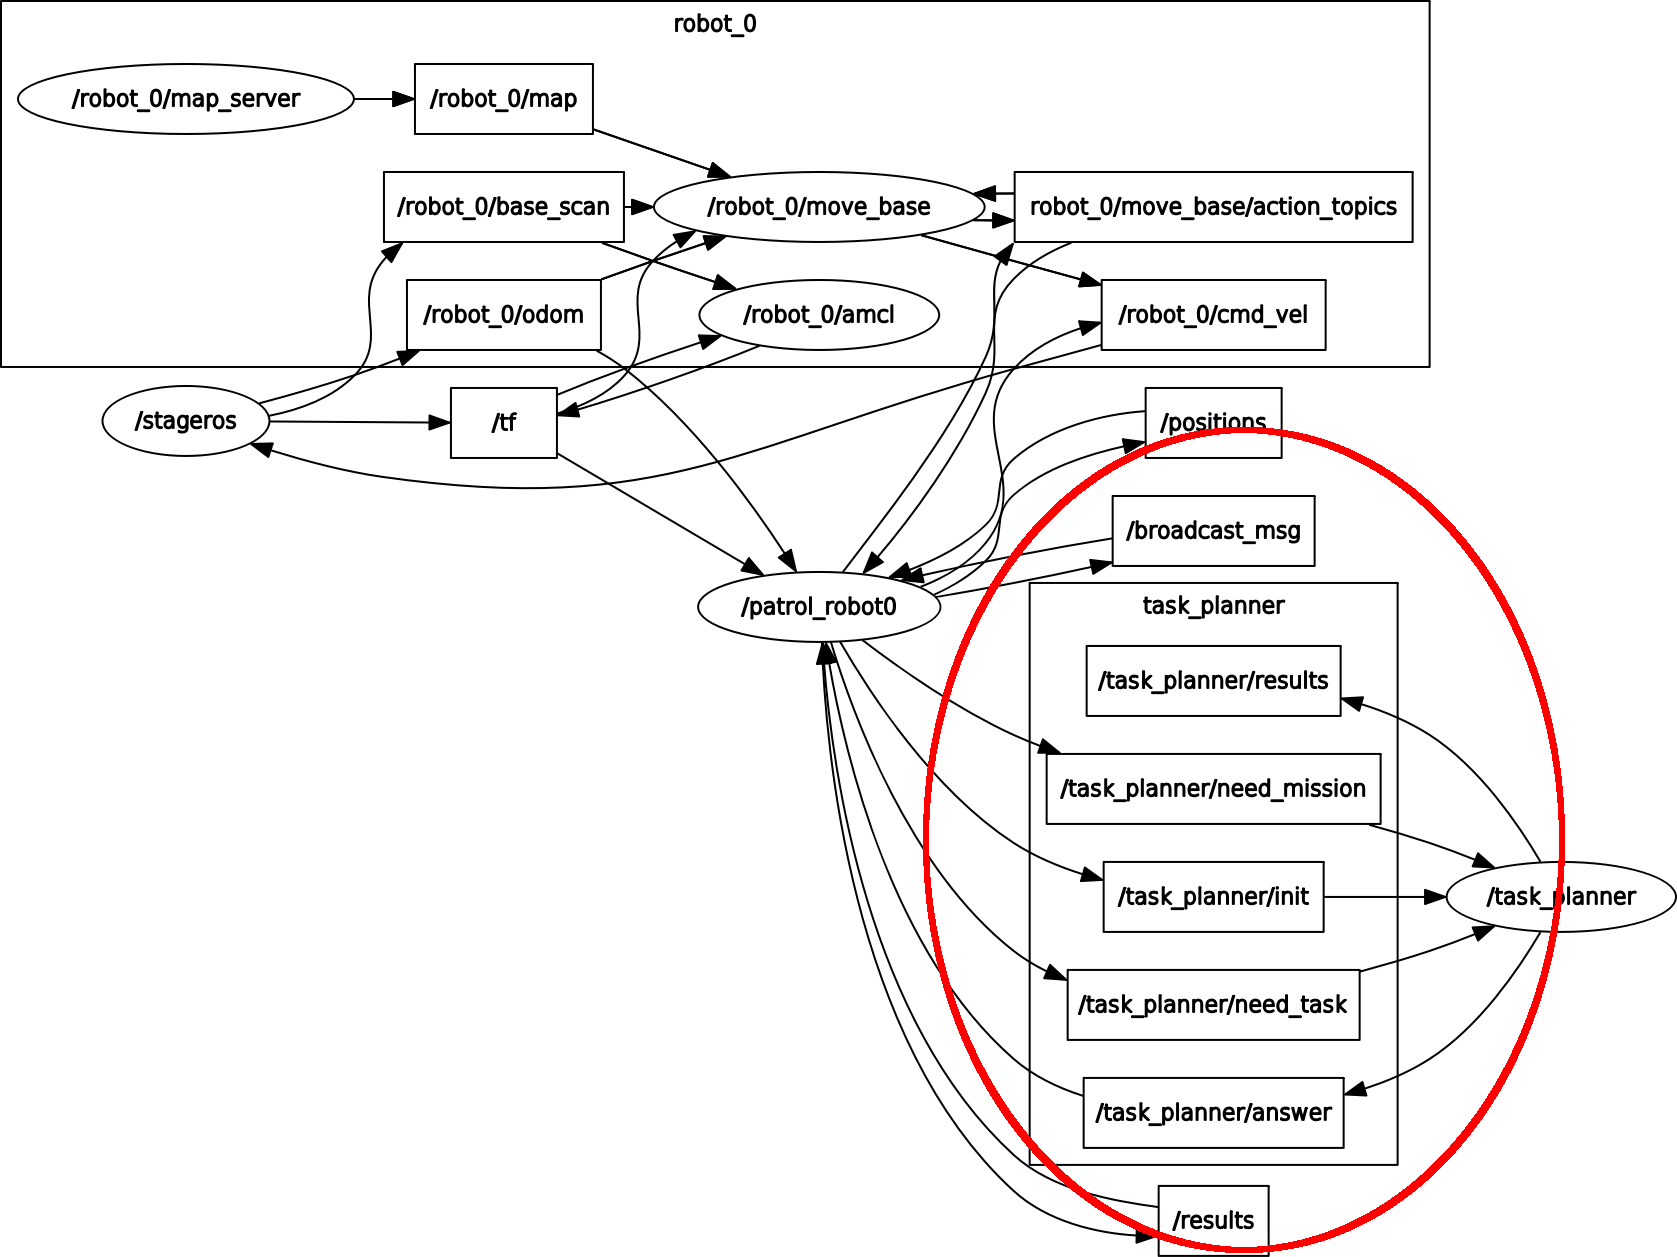
\includegraphics[scale=0.12]{img/rosgraph}
        \end{figure}
    \end{frame}

    \begin{frame}[fragile]{Empirical Results}
        \resizebox{\linewidth}{4.3cm}{
        \begin{tabular}{|c|c|c|c|c|c|} \hline
            {\bf Configuration} & {\bf Algorithm} & {\bf $ \overline{Time}$} & {\bf $\overline{Interference}$} & {\bf $\overline{Distance}$} & {\bf $\bar{\sigma}(Distance)$}         \\ \hline
            6/-/2               & \srst           & 218.32$[\pm 6.19]$        & 63.45   & 3747.90 &  87.8\\ \hline 
            6/3/2               & \gsp            & 194.52$[\pm 6.42]$        & 49.65    & 3401.15 & 251.37  \\ 
                                & \sps            & 177.00$[\pm 1.99]$        & 49.34    & 3132.5 & 0  \\ \hline
            6/5/2               & \gsp            & 142.08$[\pm 1.39]$       &   42.2        & 2714.25      &  206.43  \\
                                & \sps            & 138.98$[\pm 2.41]$       &  39.38   &  2601.25  &  156.47   \\ \hline
            6/-/4               & \srst           & 124.52$[\pm 3.12]$        & 42    & 2194.75 &  114.2 \\ \hline
            6/3/4               & \gsp            & 117.44$[\pm 1.85]$        & 35.75   & 1769 & 43.83  \\ 
                                & \sps            & 115.28$[\pm 4.10]$        & 33.5   & 1702.5 & 23.67  \\ \hline
            6/5/4               & \gsp            &  93.4$[\pm 1.01]$         & 29     & 1688.5 &  34.5   \\
                                & \sps            &  91.8$[\pm 2.14]$        & 30.75  & 1546.5 & 35.8  \\ \hline
            9/-/2               & \srst           & 292.24$[\pm 3.06]$      &  85.5  & 5201.5 & 34.76\\ \hline
            9/3/2              & \gsp            & 265.72$[\pm 2.64]$      & 71.5   & 4491.5  & 0  \\ 
                               & \sps            & 240.74$[\pm 10.42]$        & 75.5    & 4232.5 & 310.43 \\ \hline
             9/5/2             & \gsp          & 232.84$[\pm 4.71]$      &  68.85  &  4041.25  &  236 \\
                               & \sps           &168.34$[\pm 2.03]$       &   50.5   & 3132.5 &  0  \\ \hline 
            9/-/4               & \srst           & 178.55$[\pm 4.23]$     & 52  & 2755.75 & 135.8 \\ \hline
            9/3/4               & \gsp            & 152.55$[\pm 2.87]$     & 46.75 & 2200 & 113.4 \\ 
                               & \sps            & 134.23$[\pm 3.25]$     &  40.63   & 2182.5 & 27 \\ \hline
            9/5/4              & \gsp           &134.23$[\pm 3.26]$        & 40.6    & 2098.3     &   93.45    \\
                               & \sps           &93.05$[\pm 5.15]$         & 32.25    & 1530.25 &   0 \\ \hline    
            21/-/2             & \srst           & 629.10$[\pm 8.84]$        & 154.6   &11773.5 &  229.75 \\ \hline
            21/3/2              & \gsp            & 561.93$[\pm 8.00]$     &  134.3  &10133.16 &  201.2   \\ 
            21/5/2              & \gsp            & 497.45$[\pm 6.15]$      & 126  & 9079 & 210.4  \\ \hline
            21/-/4              & \srst           & 402.12$[\pm 5.06]$     & 132.25  & 6232.35 &  295.1 \\ \hline
            21/3/4              & \gsp            & 343.23$[\pm 6.10]$ & 98.23 & 5231.25 & 342.2   \\ 
            21/5/4              & \gsp            & 294.40$[\pm 7.60]$ & 77.63 & 4683.25 & 367.5  \\ \hline
        \end{tabular}}
    \end{frame}

   

    \begin{frame}[fragile]{Conclusions and Future Work}
        In conclusion: 
        \begin{itemize}
            \item Good behavior of GSP comparison a SPS.
            \item The quality of solutions found by GSP is comparable with the 
            quality of solutions found by SPS.
            \item Coalition Formation problem can approximate the results 
            of a set partion problem in {\bf less} time complexity.
        \end{itemize}
        We are focused on a {\bf centralized coordinator} in the future works we want to 
        perform a {\bf distributed coordiantion}.

        That strategy should be more {\bf flessible}, {\bf adaptive} at the situation on the traveling
        orders then {\bf fault-tolenace}. 
    \end{frame}






